\section{AWS cost}
\label{sec:AWS cost}
As already mentioned, this paragraph will be dedicated to the analysis of the costs of the various services described above.
In particular the following tables contain data collected from price lists of AWS, then these will be processed to estimate the monthly cost and yearly need for the realization of the entire platform.
The following statements are based upon some assumptions resulting from the use case of interest and allow a more rapid interpretation:

\begin{itemize}
\item The videos last on average 5 minutes
\item The size of the video changes depending on the quality:

\begin{table}[h!]
\centering
\begin{tabular}{ |p{3cm}|p{3cm}|p{3cm}|  }
  \hline
  \multicolumn{3}{|c|}{Cost for minute} \\
  \hline
  Minute & Quality & Cost \\
  \hline
  1 & SD & 0.01185185185 \\
  1 & HD & 0.08 \\
  \hline
\end{tabular}
\caption{Table of cost for minute}
\label{table:1}
\end{table}

\begin{table}[h!]
\centering
\begin{tabular}{ |p{3cm}|p{3cm}|p{3cm}|  }
  \hline
  \multicolumn{3}{|c|}{Gb for a video} \\
  \hline
  Video & Quality & Gb \\
  \hline
  1 & SD & 0.05925925926 \\
  1 & HD & 0.4 \\
  \hline
\end{tabular}
\caption{Table of Gb for a video}
\label{table:1}
\end{table}


\item The cost of transcoding service provided by Elastic Transcoder is:

\begin{table}[h!]
\centering
\begin{tabular}{ |p{3cm}|p{3cm}|p{3cm}|  }
  \hline
  \multicolumn{3}{|c|}{Elastic Transcoder cost for minute} \\
  \hline
  Minute & Quality & Cost \\
  \hline
  1 & SD & 0.0185 \\
  1 & SD & 0.037 \\
  \hline
\end{tabular}
\caption{Table of cost for minute}
\label{table:1}
\end{table}

\begin{table}[h!]
\centering
\begin{tabular}{ |p{3cm}|p{3cm}|p{3cm}|  }
  \hline
  \multicolumn{3}{|c|}{Elastic Transcoder cost for a video} \\
  \hline
  Video & Quality & Cost \\
  \hline
  1 & SD & 0.0925 \\
  1 & HD & 0.185 \\
  \hline
\end{tabular}
\caption{Table of cost for a video}
\label{table:1}
\end{table}


\item The cost of storage of video on S3 is 0.03\$/GB
\item The cost for the network traffic is:


\begin{table}[h!]
\centering
\begin{tabular}{ |p{3cm}|p{3cm}|p{3cm}|  }
  \hline
  \multicolumn{2}{|c|}{Network traffic} \\
  \hline
  TB & Cost per GB \\
  \hline
  10 & 0.09 \\
  40 & 0.08 \\
  100 & 0.06 \\
  350 & 0.04 \\
  524 & 0.03 \\
  4000 & 0.03 \\
  5000 & 0.02 \\
  \hline
\end{tabular}
\caption{Table of network traffic cost}
\label{table:1}
\end{table}


\end{itemize}

Once collected the costs of the various services used in e-learning, as mentioned previously, now we focus on the calculation of some estimates based on the number of videos and the number of views.

Total cost for storage on S3 and transcoding is:


\begin{table}[h!]
\begin{tabular}{ |p{2cm}|p{2cm}|p{2cm}|p{2cm}|p{2cm}| }
  \hline
  \multicolumn{5}{|c|}{S3 and Elastic Transcoder} \\
  \hline
  video & S3 month & S3 year & Elastic Transcoder & Total \\
  \hline
  100 & 1.2 & 14.4 & 18.5 & 32.9\\
  1000 & 12 & 144 & 185 & 329\\
  10000 & 120 & 1440 & 1850 & 3290\\
  50000 & 600 & 7200 & 9250 & 16450\\
  100000 & 1200 & 14400 & 18500 & 32900\\
  500000 & 6000 & 72000 & 92500 & 164500\\
  1000000 & 12000 & 144000 & 185000 & 329000\\
  \hline
\end{tabular}
\caption{Table of total cost per storage and transcoder}
\label{table:1}
\end{table}

Cost of video streaming in standard definition(SD) is:

\begin{table}[h!]
\begin{tabular}{ |p{2cm}|p{2cm}|p{2cm}|p{2cm}|p{2cm}| }
  \hline
  \multicolumn{5}{|c|}{SD Streaming cost} \\
  \hline
  views & minute & gb & cost/month & single video cost\\
  \hline
1,000 & 5,000 & 59.26 & 5.04 & 0.00504\\
10,000 & 50,000 & 592.59 & 50.37 & 0.00504\\
50,000 & 250,000 & 2,962.96 & 251.85 & 0.00504\\
100,000 & 500,000 & 5,925.93 & 503.70 & 0.00504\\
500,000 & 2,500,000 & 29,629.63 & 2,420.37 & 0.00484\\
1,000,000 & 5,000,000 & 59,259.26 & 4,605.56 & 0.00461\\
5,000,000 & 25,000,000 & 296,296.30 & 15,901.85 & 0.00318\\
10,000,000 & 50,000,000 & 592,592.59 & 26,827.78 & 0.00268\\
  \hline
\end{tabular}
\caption{Table of SD Streaming cost}
\label{table:1}
\end{table}


Cost of video streaming in high definition(HD) is:

\begin{table}
\centering 
\begin{tabular}{ |p{2cm}|p{2cm}|p{2cm}|p{2cm}|p{2cm}| }
  \hline
  \multicolumn{5}{|c|}{HD Streaming cost} \\
  \hline
  views & minute & gb & cost/month & single video cost\\
  \hline
1,000 & 5,000 & 400 & 34 & 0.034 \\
10,000 & 50,000 & 4,000 & 340 & 0.034\\
50,000 & 250,000 & 20,000 & 1650 & 0.033\\
100,000 & 500,000 & 40,000 & 3250 & 0.0325\\
500,000 & 2,500,000 & 200,000 & 12050 & 0.0241\\
1,000,000 & 5,000,000 & 400,000 & 20050 & 0.02005\\
5,000,000 & 25,000,000 & 2,000,000 & 64170 & 0.012834\\
10,000,000 & 50,000,000 & 4,000,000 & 114170 & 0.011417\\
  \hline
\end{tabular}
\caption{Table of HD Streaming cost}
\label{table:1}
\end{table}

The data illustrated above can be synthesized through the use of a few charts:

\begin{figure}[htb]
 \centering
 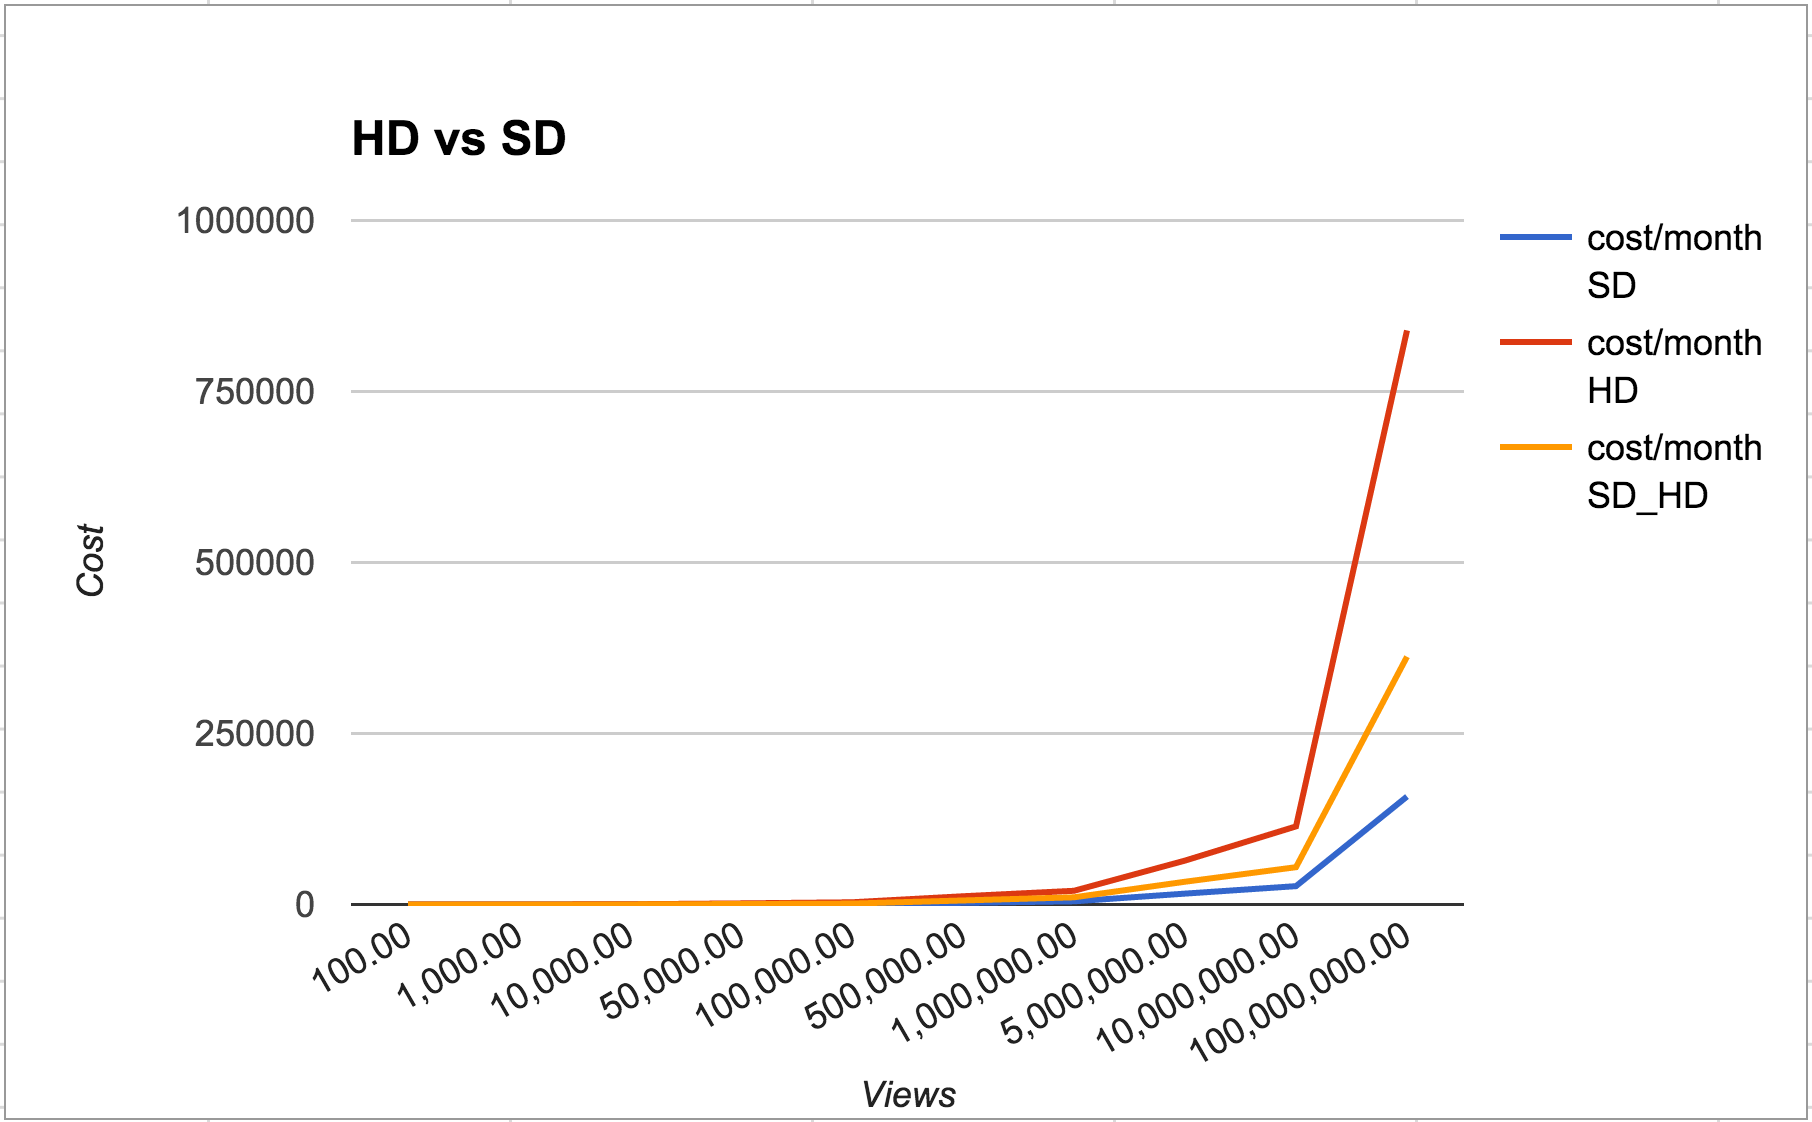
\includegraphics[width=1.0\linewidth]{images/chapter2/grafico.png}\hfill
 \caption[Comparison of monthly costs]{Comparison of monthly costs}
 \label{fig:fourV}
\end{figure}
